%!TEX root = ../thesis.tex
\externaldocument[A-]{Chapters/appendix.tex}

\part{Muxmon experiment}
  \textbf{large TODO:}
  \begin{itemize}
    \item Explain surface code architecture
    \item Explain the general structure of a chip:
    \begin{itemize}
      \item Feedline through which signal is sent and measured
      \item CPW resonators, capacitively coupled to feedline
      \item Single qubit coupled to resonators (coupling location?)
      \item Resonator buses
    \end{itemize}
  \end{itemize}

  \textbf{small TODO:}
  \begin{itemize}
    \item Rename DAC voltage to flux, and mention early on that this renaming will be used
    \item flux-bias line or flux bias line?
  \end{itemize}



  \chapter*{Introduction}

    At this moment circuit QED is at the stage where multi-qubit experiments are being realized.

    \begin{itemize}
        \item Scaling up
        \item Challenges involved in scaling
        \item Frequency re-use, Duplexer intro
    \end{itemize}





  \chapter{Qubit characterization}
    \begin{description}
     \item[Description] This chapter gives a step-by-step description of how to find a resonator and qubit, and subsequently how to tune the qubit's parameters.
     \end{description}

    In the design of cQED chips, the parameters of the qubits and resonators are always targeted which are ideal for the experiment.
    For coplanar waveguide resonators one can already obtain relatively good parameters for the required dimensions from simple formulae \textbf{TODO:} refer to formula.
    For superconducting transmon qubits, however, finding the right dimensions that correspond to the desired parameters is a much more complicated process.
    The qubit's frequency, for instance, depends on the qubit's coupling energy $\Ec$ and Josephson energy $\Ej$. The coupling energy $\Ec$ can be reasonably estimated from classical simulations. Finding the right dimensions for the Josephson junction that result in the desired Josephson energy $\Ej$, however, is difficult, and usually physically testing different junctions is necessary to determine an accurate conversion from the desired $\Ej$ to the Josephson junction dimensions.

    Nevertheless, the actual parameters of the resonators and qubits are almost never where one expects them to be. Once the sample is cooled in the dilution refrigerator, an inevitable game of hide-and-seek follows with the goal of finding the frequency of the resonators and qubits, and subsequently determining their properties. This chapter describes the measurements that were performed to characterize the MuxMon samples.

    \section{Continuous-wave measurements}

      Once a sample is properly cooled down it is ready to be measured. At this stage the sample is still an unknown terrain, where the experimenter only has a rough map, containing the sample's targeted parameters, and the specific properties of the resonators and qubits.

      The first step is to look for signs of life. These manifest themselves as resonance frequencies of the resonators and the qubits that are coupled to them. As we are not yet interested in the properties of the resonators and qubits which can only be obtained through measurements with accurately timed pulses, we send continuous tones through the feedline, and measure deviations in the transmission. These measurements are known as continuous-wave measurements

      \subsection{Scanning for resonators}
        \label{sec:resonator-scan}
        Since communication with the qubits is mediated through their coupling to resonators, the first step is to find these resonators. This is done using a transmission measurement, in combination with heterodyne detection, and has been explained in section \textbf{TODO:} Create section in Resonator chapter.

        There is one difference in measuring a resonator when there is a qubit coupled to it. When considering the qubit as a two-level system, the behaviour of the coupled resonator-qubit system is governed by the Jaynes-Cummings Hamiltonian \cite{Reed}:

        \begin{equation}
          \hat{H} = \hbar \wres\left(\hat{a}^\dagger \hat{a} + \frac{1}{2} \right) + \frac{\hbar \wqub}{2}\hat{\sigma}_z + \hbar g \left(\hat{a}^\dagger \sigma_{-} + \hat{a}\sigma_{+}\right)
          \label{eq:Jaynes-Cummings}
        \end{equation}

        where $\wres$ is the bare resonance frequency of the resonator, $\wqub$ is the resonance frequency of the qubit's ground to excited state transition, and the qubit's two states are in the spin-representation. This Hamiltonian consists of three terms. The first term corresponds to the energy level of the resonator, the second to the energy level of the transmon, and the third is a coupling term between the two with coupling strength $g$.

        The difference between the resonator's frequency $\wres$ and the qubit's frequency $\wqub$ is given by the detuning $\Delta = \wqub - \wres$. If the magnitude of the detuning is large compared to the coupling strength $g$, the system is in the dispersive regime. In this case the Hamiltonian can be approximated by the dispersive Jaynes-Cummings Hamiltonian:

        \begin{equation}
          \hat{H} = \frac{\hbar \wqub^{'}}{2} \hat{\sigma}_z +  \left(\hbar \wres^{'} + \hbar \chi \hat{\sigma}_z\right) \hat{a}^\dagger \hat{a}
          \label{eq:dispersive-Jaynes-Cummings}
        \end{equation}

        The coupling between the qubit and resonator causes both qubit's frequency and the resonator's frequency to shift: $\wqub^{'} = \wqub + \chi_{01}$, $\wres^{'}=\wres - \chi_{12}/2$.

        Aside from experiencing a frequency shift dependent on the amount of detuning, Equation~\ref{eq:dispersive-Jaynes-Cummings} shows that the resonator also experiences a shift depending on the state of the qubit. The resonator's frequency is decreased by an amount $2 \chi$ when the qubit is in the excited state. The parameter $\chi$ is the dispersive shift, and is given by:

        \begin{equation}
          \chi = \chi_{01} - \chi_{12}/2 \approx \frac{g^2}{\Delta}\frac{\Ec}{\hbar \Delta - \Ec}
          \label{eq:dispersive-shift}
        \end{equation}

        where $\chi_{ij} = \frac{g_{ij}^2}{\omega_{ij}-\omega_c}$ are the partial dispersive shifts.

        Due to this coupling between resonator and qubit, it is important to choose the right RF power. When the amount of photons in the resonator reaches a certain point, this coupling will result in the resonator experiencing nonlinear effects. The resonator will thereby lose its Lorentzian lineshape. Therefore the RF power should be kept sufficiently low to avoid these nonlinear effects, while still maintaining a good signal-to-noise ratio.



        \textbf{TODO:}
        \begin{itemize}
          \item In the strong coupling regime (Leads to hybridization of qubit and resonator states: quton and fobit
          \item Explain that the quality factor is low because the resonator is coupled strongly to the qubit (equation including coupling to qubit?)
          \item Doesn't $\chi$ diverge when $\Delta \rightarrow \Ec$?
          \item explain concept of anharmonicity, and that $\alpha \approx E_c$
          \item Maybe explain concept of number splitting in dispersive Jaynes-Cummings. Number splitting is the phenomenon that the qubit's frequency shifts by an amount $2 \chi$ for every photon in the resonator.\\
                Alternatively mention this in another section.
          \item Mention that $g_{12}=\sqrt{g}$, and that other coupling strengths are exponentially suppressed in the transmon
        \end{itemize}

        \textbf{Figures:}
        \begin{itemize}
          \item Figure of transmission showing all three Muxmon0 resonators
        \end{itemize}

      \subsection{Powersweeping the resonators}
        Once the resonators have been located, the next stage is to find the qubit that is capacitively coupled to each of the resonators. Instead of directly scanning the entire frequency spectrum in search of the qubit, it is relatively straightforward to perform some initial measurements aimed at gaining information about our resonator and qubit, which will allow us to search for our qubit with much greater accuracy.

        As explained previously, the capacitive coupling between the resonator and qubit shifts the resonator frequency $\wres$ from its bare frequency. When the amount of photons in the resonator reaches a certain point, the resonator experiences nonlinearity, thereby losing its Lorentzian lineshape. When increasing the RF power even further, at a certain point the resonator regains its Lorentzian lineshape. In doing so its resonance frequency has shifted to its bare frequency $\wbare$. If this frequency shift is observed, it indicates that the resonator's frequency was shifted, and hence that the qubit is alive. Measuring this frequency shift is commonly done in a powersweep. A powersweep is a measurement in which a resonator scan is performed for a range of powers.

        A powersweep additionally provides information about at what power the resonator enters the nonlinear regime. For measurements involving the qubit the readout power must be below this threshold power. Furthermore, from the frequency shift between the dressed cavity frequency and the bare cavity frequency, the amount of detuning between the qubit and the resonator can be estimated using Equation~\ref{eq:dispersive-shift}.

        If no shift is observed, it could mean that the qubit is dead (e.g. because the Josephson junction is shorted). However, this is not necessarily the case. An alternative possibility is that the detuning between qubit and resonator is very large, and as a result the frequency shift cannot be discerned. At this point it is too early to draw conclusions, and we may almost draw the analogy with Schr\"odinger's cat in a box.

        \textbf{TODO:}
        \begin{itemize}
          \item Explain theory behind transition to bare cavity frequency (Reed's thesis has some information)
        \end{itemize}

        \textbf{Figures:}
        \begin{itemize}
          \item Powersweep of ancilla qubit
        \end{itemize}

      \subsection{Scan for qubit sweet-spots}
        Some of the qubits have a tunable resonance frequency. This is done through a superconducting quantum interference device (SQUID). In this case the two islands that compose the transmon qubit are connected by two Josephson junctions instead of one, effectively forming a loop. The SQUID loop is sensitive to the amount of flux passing through the loop. The amount of flux going through the SQUID loop can be changed by changing the surrounding magnetic field. This is commonly done by having a flux bias line in close proximity to the SQUID loop. Current flowing through the flux-bias line alters the magnetic field in the vicinity of the SQUID loop, and hence changes the amount of flux through the SQUID loop. A digital-to-analog converter is used to specify the amount of current that is sent through the flux bias line. Depending on the amount of flux through the SQUID loop, the resonance frequency of the qubit changes accordingly. these qubits are therefore called flux-tunable.

        For qubits that are flux-tunable, finding the sweet-spot of the qubit can be done without knowledge of the qubit's frequency. This can be done by sweeping the DAC voltage and measuring the shift in the resonance frequency. Because the frequency of the qubit varies as the amount of current through the flux-bias line changes, the detuning between the qubit and the resonator consequently changes. As a result the dispersive shift $\chi$, and therefore the resonator's frequency, also varies. At the sweet-spot of the qubit, the resonator's frequency $\wres$ is at a maximum. This is irrespective of whether the qubit's frequency $\wqub$ is above or below the resonator's frequency.

        The accurate way to measure the sweet-spot is to perform resonator scans as the DAC voltage is varied. The result is a 2D scan shown in \textbf{TODO:} Figure.

        A faster second approach for finding the qubit sweet-spot, at the cost of providing less information, is by choosing a fixed frequency close to the resonator's frequency $\wres$ (preferrably slightly below, where the transmission slope is steepest). By measuring the amount of transmission as the DAC voltage is being varied, one obtains essentially a line-cut of \textbf{TODO:} Figure. The idea this measurement is that if the qubit's frequency $\fqub$ decreases, the resonator's frequency also decreases, resulting in a decrease in transmission (closer to $\wres$). Likewise, if the qubit's frequency $\wqub$ increases, the resonator's frequency increases \textbf{TODO:} Why?, resulting in an increase in transmission (further away from $\wres$).

        At the qubit's sweet-spot, the resonator's frequency $\wres$ is at a maximum, and so the transmission should also be at a maximum. Furthermore, because the amount of detuning only depends on the deviation from the flux sweet-spot \textbf{TODO:} improve, the transmission should be symmetric with respect to the DAC voltage sweet-spot. If the resonator's frequency $\wres$ shifts by a large amount in the course of this measurement, it becomes harder to determine where the sweet-spot is (although even then often it can still be discerned). Nevertheless, this method is considerably faster than performing a full two-dimensional scan of frequency versus DAC voltage, and in most cases it works like a charm.

        In the case where the powersweep showed no measurable frequency shift, these two measurements are also useful in discerning whether or not the qubit is actually dead, or whether it was simply far detuned from the resonator.


        \textbf{TODO:}
        \begin{itemize}
          \item Explain how qubit's frequency has a cosine dependence on DAC
          \item Give detailed information on SQUID loop
          \begin{itemize}
            \item Why does the qubit frequency change in a SQUID loop
            \item Sweet-spot
          \end{itemize}
          \item Mention flux-noise?
          \begin{itemize}
            \item 1/f noise
            \item usually not limiting, as it is very slow
            \item This noise can be seen as occasional jumps (every few hours?) It would mean that every few hours the frequency must be recalibrated.
          \end{itemize}
        \end{itemize}

        \textbf{Figures:}
        \begin{itemize}
          \item SEM picture of SQUID loop, including flux-bias line
          \item Figure of 2D resonator scan vs DAC voltage
          \item Figure of 1D resonator fixed frequency DAC voltage scan
        \end{itemize}

      \subsection{Scanning for qubits}
        \label{sec:spectroscopy}
        Once the preliminary measurements have been performed that characterize the resonators and provide hints about the whereabouts of the qubit it is time to actually find the qubit.

        The measurement to perform in order to find the qubit depends on the amount of detuning between the resonator and qubit, which can be estimated from powersweep measurements. If the amount of detuning is large compared to the coupling strength ($\Delta \gg  g$), the system is in the dispersive regime. In this case one commonly performs a two-tone spectroscopy to find the qubit's frequency. If, on the other hand, the detuning is comparable to the coupling strength ($\Delta \sim g$), the qubit and resonator are hybridized, and experience an avoided crossing. In such cases a normal transmission measurement suffices.

        If the qubit is flux-tunable, one important question to ask is: at what DAC voltage should the qubit be searched?

        One option is to choose zero DAC voltage. In most cases this is alright, but there are cases when this is a bad choice. For instance, trapped magnetic fields during cool-down could position the qubit near the anti-sweet-spot for zero DAC voltage, in which case finding the qubit will be next to impossible.

        A better option is to choose a DAC voltage that results in a detuning $\Delta$ that is large compared to coupling strength $g$, such that the system is in the disperisive regime. However, the detuning $\Delta$ should not be too high, as it would otherwise result in a negligible dispersive shift $\chi$.The optimum value is usually around a few hundred megahertz, although this is dependent on the device-specific parameters. The detuning can be approximated using powersweeps.

        \subsubsection{Spectroscopy}
          As was explained in section~\ref{sec:resonator-scan}, in the dispersive regime the resonator experiences a $2 \chi$ frequency shift dependent on the state of the qubit. In the case of a resonator capacitively coupled to the feedline, the transmission experiences a dip at the resonator's frequency. This dip will correspondingly shift when the qubit's state is switched. The transmission at the resonator's dip when the qubit is in the ground state will therefore be dependent on the state of the qubit (low when the qubit is in the ground state, high when the qubit is in the excited state). This is the property exploited in a two-tone spectroscopy measurement.

          In a two-tone spectroscopy measurement two tones are sent through the feedline.
          \begin{enumerate}
            \item A drive tone with varying frequency $\wdrive$.
            \item A measurement tone at the resonator's frequency when the qubit is in the ground state.
          \end{enumerate}

          The transmission through the feedline is measured while the frequency of the drive tone $\wdrive$ is swept. When the drive frequency $\wdrive$ is detuned from the qubit's frequency $\wqub$, the drive is off-resonant with respect to the qubit, and so we measure a low transmission due to a dip being present. However, when the drive frequency $\wdrive$ approaches the qubit's frequency $\wqub$, then the qubit will start to oscillate between its ground and excited state, with a rate dependent on the detuning between the drive frequency $\wdrive$ and the qubit's frequency $\wqub$. The qubit will therefore have a partial population in the excited state, resulting in a shift of the resonator frequency, dependent on the population in the excited state. This is measured as an increase in transmission.

          The minimum linewidth of the qubit using spectroscopy is set by its dephasing time $T^2$, which can be seen as the uncertainty in its frequency. However, the power of the drive tone causes an additional increase in the linewidth, due to stimulated emission of the qubit. This effect is known as power broadening. This effect can be quite useful for finding qubits, especially when designing high-quality qubits with a very narrow intrinsic linewidth. The optimal power for the drive strength is further dependent on the amount of detuning $\Delta$ between the qubit and resonator. The resonator effectively acts as a bandpass filter, centered around the resonator frequency. Therefore, the stronger the detuning, the more the drive tone is suppressed.

          The dispersive shift $2 \chi$ is also dependent on the amount of detuning $\Delta$ between the qubit and resonator. If the detuning $\Delta$ is large, the dispersive shift will be very small, and so the difference in transmission will also decrease. Since the resonator has a Lorentzian lineshape, at the resonance frequency this Lorentzian is flat, and so is insensitive to small deviations. To increase the contrast between the on-resonant and off-resonant transmission, it is usually advantageous to measure at a slight detuning $\delta$ away from the resonance frequency, where the transmission slope is high. Since the resonator frequency shifts down when the qubit is excited, it is better to have a positive detuning $\delta$ to ensure that the transmission increases as the drive frequence $\wdrive$ approaches the qubit frequency $\wqub$ and decreases as it leaves the qubit frequency.

          \textbf{TODO:} Spectroscopy section
          \begin{itemize}
              \item Is power broadening really due to stimulated emission?
              \item Explain optimal RF power
              \item Is the gradual increase really due to partial population? Is it then an average of the partial population? Or do you get other effects as well?
          \end{itemize}


        \subsubsection{Avoided crossing}
          When the detuning $\Delta$ between the qubit and resonator is not large compared to their coupling strength $g$, the qubit and resonator experience an avoided crossing. Because all of the qubits in the Muxmon chips are considerably lower in frequency compared to their resonators, the system is always in the dispersive regime, and so the system never approaches the avoided crossing. Nevertheless it is worth mentioning the avoided crossing briefly, as it is a breeding ground for interesting physics.

          At the avoided crossing the system is not in the dispersive regime, and so the dispersive Jaynes-Cummings Hamiltonian no longer applies. In this case the resonator and qubit are hybridized, and one can no longer speak of a qubit and resonator as separate entities. Instead, this hybridization results in a so-called quton and phobit.

          \textbf{Avoided crossing info:}
          \begin{itemize}
            \item The coupling strength $g$ is the minimum distance be~tween the splitting
            \item From Reed's thesis p.63 explanation of this avoided crossing is given\\
            \begin{align}
             E_0 = & -\frac{\hbar \Delta}{2}\\
             E_1 = & n \hbar\omega_r \pm \frac{\hbar}{2}\sqrt{4g^2n + \Delta^2}
            \end{align}\\
            Joining $E_0 + E_1$ results in a qubit approaching a resonator from the top.\\
            When the frequency of the qubit equals that of the resonator, the energy difference reaches a minimum, and is equal to $2g$.
          \end{itemize}

          \textbf{TODO:} Avoided crossing
          \begin{itemize}
            \item Explain the quton fobit behaviour near the avoided crossing
            \item Explain how one can extract coupling from avoided crossing
            \item Explain that for the Muxmon qubit this effect is not present
            \item Explain multiple lines near avoided crossing
          \end{itemize}

          \textbf{figures:}
          \begin{itemize}
            \item Figure of avoided crossing
          \end{itemize}


        \textbf{TODO:}
        \begin{itemize}
          \item Use relatively high source power, results in power broadening
          \item Mention what to do if qubit is close to or far away from resonator
          \item Mention the term transmission measurement earlier on.
          \item Pulsed spectroscopy
        \end{itemize}

      \subsection{Tracking the qubits}
        \label{ssec:tracked spectroscopy}
        For flux-tunable qubits one is usually not interested in finding the frequency at one specific flux value. More important is finding how this frequency changes with varying flux. A naive approach would be to perform a two-dimensional scan of a fixed frequency range versus flux. At a certain flux the qubit crosses the boundary of the chosen frequency window. Every time this happens a new two-dimensional scan has to be performed with an updated frequency window. The larger the chosen frequency window, the less often this has to be updated. On the other hand, choosing a large window also means that a larger portion of the scan is spent not measuring the qubit. There is therefore a trade-off between measurement time and degree of human intervention. Furthermore, the resonator frequency also depends on the amount of detuning. Therefore the frequency of the measurement tone must also be updated every now and then.

        As an alternative approach I have created a modified version of the spectroscopy versus flux scan, known as tracked spectroscopy. In this approach after every spectroscopy scan the qubit frequency is extracted through fitting. From the qubit frequencies measured in previous scans the expected frequency at the next flux value is extrapolated. The frequency window of the next spectroscopy scan are then centered around the expected qubit frequency. The qubit is therefore tracked as its frequency changes. The same method is applied to update the resonator frequency.

        Tracked spectroscopy has several advantages over the two-dimensional spectroscopy versus flux scans. First of all, since the qubit's frequency follows a smooth curve (see Equation~\textbf{TODO:} Refer to eqn), the qubit's frequency can be estimated quite accurately. The frequency windows can therefore be narrow. This greatly reduces the measurement time. Secondly, tracked spectroscopy does not need any human intervention, as the frequency window is automatically updated after every spectroscopy scan. Therefore measuring the flux-dependence of the qubit frequencies is an automatized process (provided that the qubit frequency can correctly be extracted).

        For more information on the tracked spectroscopy algorithm see appendix~\ref{sec:Tracked spectroscopy}.

        \textbf{Improvements}
        \begin{itemize}
          \item Avoided crossing
          \item Variable RF and drive power
        \end{itemize}
        \textbf{TODO:}
        \begin{itemize}
          \item Maybe mention possible improvements
        \end{itemize}
        \textbf{Figures:}
        \begin{itemize}
          \item Tracked spectroscopy of qubit and resonator
        \end{itemize}

      \subsection{Finding the qubit's second transition}
        \label{ssec:12-transition spectroscopy}
        Once the qubit's grequency is known, it is possible to find the qubit's excited-state to second-excited-state transition $\omega_q^{12}$, which shall be referred to as the 12-transition. For consistent notation we shall temporarily denote the qubit's ground-state to excited-state transition frequency as $\omega_q^{01}$. The anharmonicity $\alpha$ is then given by the difference in transition frequencies: $\alpha = \omega_q^{12} - \omega_q^{01}$. Knowledge of the anharmonicity $\alpha$ allows determination of the coupling energy $E_c$ through \textbf{TODO:}.

        The 12-transition can be found using three-tone spectroscopy, in a manner similar to two-tone spectropscopy measurement explained in section~\ref{sec:spectroscopy}. The following three tones are used in three-tone-spectroscopy:

        \begin{enumerate}
          \item A drive tone with fixed frequency $\omega_\text{drive}^{01}$ at the qubit frequency $\omega_q^{01}$.
          \item A drive tone with varying frequency $\omega_\text{drive}^{12}$ to scan for the 12-transition.
          \item A third tone at the resonator frequency when the qubit is in the excited-state.
        \end{enumerate}

        The first drive tone with frequency $\omega_\text{drive}^{01}$ is used the drive the qubit to the excited-state. Since the first drive tone results in the excited-state being (partially) populated, the second tone with frequency $\omega_\text{drive}^{12}$ is then able to drive the qubit from the excited-state to the second-excited-state. The transmission should therefore change when $\omega_\text{drive}^{12}$ is on resonance with $\omega_q^{12}$.

        In principle the first drive tone with frequency $\omega_\text{drive}^{01}$ can be kept fixed at the 01-transition frequency $\omega_q^{01}$. However, by performing a two-dimensional scan, where $\omega_\text{drive}^{01}$ is also varied in a small region around $\omega_q^{01}$, the 12-transition becomes much clearer. This can be seen in \textbf{TODO:} Figure. Here a shift in transmission is observed when $\omega_\text{drive}^{01} = \omega_q^{01}$. This corresponds to the 12-transmission frequency $\omega_q^{12}$. Additionally, a transmission shift is observed at a line crossing $\omega_q^{12}$. At this line $\omega_q^{01} + \omega_q^{12} = \omega_q^{02}$, resulting in some population in the second-excited state.

        Once the 12-transition transition is found, and hence the qubit's anharmonicity $\alpha$, it is the possible to calculate the coupling energy $E_c$. \textbf{TODO:}.

        Finding the resonator frequency when the qubit is in the excited-state can be tricky, as pulsed spectroscopy is usually required. Nevertheless a rough estimation can be found using a modified version of spectroscopy, where the drive tone $\omega_\text{drive}$ is kept fixed, whilst the resonator frequency is swept. The lower peak will be a rough estimation of the resonator frequency when the qubit is in the excited-state. Alternatively it is also possible to use the resonator frequency when the qubit is in the ground-state, although this will reduce the contrast between driving on-resonance and driving off-resonance.

        It is worthwhile to note that three-tone spectroscopy produces much more accurate results when using pulsed spectroscopy, as the difference in transmission is generally small compared to two-tone spectroscopy.


        \begin{itemize}
           \item Coupling energy through solving Hamiltonian (see \cite{Reed}) .
        \end{itemize}

      \subsection{Flux matrix}
        \label{ssec:Flux matrix}
        When a current is passed through a flux-bias line, it is not only the flux through the SQUID of the qubit directly connected to it that is affected. Instead, the flux through SQUIDs of neighbouring qubits are also affected, albeit to a lesser extent. Therefore changing the frequency of one qubit by changing its corresponding flux-bias line current also affects the frequencies of the other flux-tunable qubits on the chip. For the Muxmon experiment the frequencies of the three qubits have to be individually tuned to very specific frequencies, and so the frequency responses of the qubits have to be decoupled. This is done by implementing a flux matrix, which corrects for the flux cross-coupling effects.

        A flux matrix $\boldsymbol{F}$ is an $n \times n$ matrix, where $n$ is the number of flux-tunable qubits. Each row corresponds to a virtual flux, and can be interpreted as follows: in a row $F_i = \left[f_{i1}, \dots, f_{in}\right]$ each element $F_{ij}$ corresponds to the relative amount by which the flux-bias line of qubit $j$ should be changed, such that only the frequency of qubit $i$ changes, whilst the frequencies of the other qubits remain fixed. This results in $n$ decoupled virtual flux parameters.

        Creating a flux matrix is done by first determining for each qubit separately how much every flux-bias line affects its frequency. For a given qubit $i$ this can be found by tuning the qubit away from its sweet-spot using its main flux-bias line, to a point where the slope $\partial f_i/\partial V_i$ of the qubit frequency $f_i$ as a function of DAC voltage $V_i$ is steep. This is the region where we are sensitive to changes in qubit frequency. For the main flux-bias line we already know from tracked spectroscopy what the slope $\partial f_i / \partial V_i$ is at this point. For each of the remaining flux-bias lines we measure the slope $\partial f_i / \partial V_j$ as we vary the DAC voltage $V_j$ and measure the response of the qubit frequency $f_i$. The slope $\partial f_i / \partial V_j$ is a measure for the amount of flux cross-coupling, which should be considerably less than for the main flux-bias line. Finally dividing all the slopes by the slope $\partial f_i / \partial V_j$ of our main flux-bias line, results in the ratio's of the frequency response of qubit $i$ for each of the flux-bias lines. Performing this measurement for all the qubits results in a matrix $\boldsymbol{M}$, where each element $M_{ij}=\partial f_i / \partial V_j$ is the normalized frequency response of qubit $i$ when varying the DAC voltage of the flux-bias line corresponding to qubit $j$. The diagonal elements of matrix $\boldsymbol{M}$ should be equal to one.

        Tracked spectroscopy provides accurate information on the DAC voltage corresponding to the sweet-spot of a qubit. The sweet-spot may not lie exactly at zero DAC voltage. It may shift due to magnetic flux being trapped during the cooldown of the fridge. These sweet-spots are usually found in the case where all the remaining flux-bias lines are set to zero DAC voltage. There is a certain combination of DAC voltages $\vec{V}^{ss}$ for which all the qubits are at their simultaneous sweet-spot. This simultaneous sweet-spot can be found using matrix $\boldsymbol{M}$. We know for each qubit $i$ the DAC voltage $V^0_i$ corresponding to its sweet-spot. Since $\boldsymbol{M}$ stores the amount by which each flux-bias line affects the flux of any qubit, the qubit $i$ remains at its sweet-spot as long as $\boldsymbol{M}_i \vec{V}=V^0_i$ holds, where $\vec{V}$ is the vector containing the DAC voltages. Therefore the simultaneous sweet-spot $\vec{V}^{ss}$ can be found by solving the set of equations $\boldsymbol{M} \vec{V}^{ss} = \vec{V^0}$, where $\vec{V}^0$ contains the DAC voltages of the individual sweet-spots of the qubits.

        The flux matrix $\boldsymbol{F}$ can be found by inverting matrix $\boldsymbol{M}$. As mentioned earlier, each row of matrix $\boldsymbol{F}$ corresponds to the ratio by which the DAC voltages of the flux-bias lines need to be varied, such that the frequency of only one qubit is changed. We may therefore multiply each row by a different constant, as long as the ratio between the elements in each row stays constant. One can normalizing each row such that the main flux-bias line is equal to one. This has the advantage that there is a one-to-one correspondence between DAC voltage and flux, and as a result the tracked spectroscopy will look identical. Additionally, after the normalization each row can be multiplied by a factor such that the virtual flux is equal to the flux quanta present in the SQUID loop. This conversion factor can be obtained by fitting the qubit frequency curve obtained from tracked spectroscopy.

        For a given virtual flux vector $\vec{\Phi}=\left[ \phi_1, \dots \phi_n \right]$, the corresponding DAC voltages $\vec{V}$ are given by:

        \begin{equation}
          \vec{V} = \boldsymbol{F} \vec{\Phi} + \vec{V}^{ss}
        \end{equation}

        By adding the simultaneous sweet-spot DAC voltages $\vec{V}^{ss}$, we obtain the additional property that the sweet-spot of the virtual fluxes is set to zero.

        After determining the flux matrix $\boldsymbol{F}$, there will still be some small remaining cross-coupling, which depends on the accuracy of the measurements. The process of creating a flux matrix can then be repeated, but instead of using DAC voltages as the varying parameters to construct matrix $\boldsymbol{M}$, the virtual fluxes should be used. Furthermore, as the cross-coupling is small compared to before, the flux range can be much greater, such that small slopes can be accurately measured. The resulting flux matrix $\boldsymbol{F}_2$ can then simply be multiplied with the first flux matrix $\boldsymbol{F}$ to obtain a more accurate final flux matrix.

    \section{Time-domain measurements}
      \subsection{Qubit control}
        So far the measurements described have all dealt with continuous tones being applied and measuring the response in the transmission. These are crude measurements, that are nevertheless able to determine some properties of the qubit and resonator, such as their frequencies. However, to find more detailed properties of the qubits, such as their coherence times, one cannot apply a continuous tone, that drives some incoherent qubit population. Instead well-calibrated pulses are required, which modify the state of the qubit in a precise manner, corresponding to gates being applied to the qubit. These types of measurements are called time-domain measurements, as they require precise pulse timing.

        A simple time-domain measurement usually consists of two parts. The first part consists of controlling the qubit. Here pulses are sent which modify the state of the qubit. The second part consists of measuring the state of the qubit. This is done through a readout tone, similar to spectroscopy measurements. This readout tone projects the state of the qubit onto the Z-axis. From the response in the transmission the state of the qubit can be inferred. More complicated experiments may involve some sort of feedback loop, where additional qubit control can be applied depending on the measurement outcome. These measurements require the qubit readout to be quantum non-demolition, i.e. the state of the qubit is not destroyed in the process of qubit readout. This usually involves extremely low-noise amplification, such as through a Josephson parametric amplifier. Feedback measurements are not performed in this experiment, and are therefore beyond the scope of this thesis.

        Qubit pulses usually have a Gaussian shape. These pulses can be generated by modulating a carrier signal from an RF generator, and is commonly done using an Arbitrary Waveform Generator (AWG). For the Muxmon experiment the Tektronix AWG5014 is used, which has four channels, each of which can control its voltage output at the nanosecond scale. It further has eight marker channels, which can be used to trigger devices, such as RF generators and the Duplexer. The carrier signal is sent through the LO port of the mixer, and an AWG channel is connected to the IF port of the mixer. The ouput at the RF port of the mixer is the modulated signal, the amplitude of which depends on the amplitude of the AWG channel output.

        For IQ mixers it is also possible to modulate both quadratures of the carrier signal independently, using two AWG channels. This allows for single sideband modulation, which is done by convoluting the pulses of the I and Q quadrature channels with a sine and cosine respectively. The sideband modulation frequency $\omega_{sb}$ of these sinusoidal functions is the amount by which the carrier signal is shifted. Single sideband modulation has the advantage that the carrier frequency $\omega_c$ is shifted away from mixer leakage, which would otherwise cause a slight continuous rotation of the qubit. For more information on mixer leakage, see section~\ref{sec:Mixer calibration}.

        The length of the pulse is an important consideration. Shorter pulses allow for more qubit operations within its coherence time. On the other hand, the shorter a pulse is in time, the larger its frequency spectrum will be. At a certain point the spectrum will be so broad that there will be a nonnegligible signal at the qubit's excited-state to second excited-state transtion frequency. This will cause leakage to the second excited-state, thereby leaving the two-state Hilbert space.
        Furthermore, the finite resolution of the AWG causes the pulses to be discretized, resulting in the pulses being slightly distorted. The shorter the length of the pulse, the more discretization, and therefore distortion, will occur. This can cause further leakage to the second excited-state. It is therefore desirable to have a bandwidth, which is the inverse of the width $\sigma$ of the Gaussian pulse, that is small compared to the anharmonicity of the qubit.

        A second pulse, known as the Derivative Removal by Adiabatic Gate (DRAG) pulse \cite{motzoi2009simple}, can be applied along with the main pulse, to reduce the amount of leakage. The DRAG pulse is the derivative of the main Gaussian pulse, and adiabaticaly populates the second excited state during the pulse, and subsequently withdraws this population back to the two-state Hilbert space. Using the DRAG pulse can reduce the amount of leakage by orders of magnitude.

        \textbf{TODO:}
        \begin{itemize}
          \item Explain about the measurement process, and that many averages need to be performed to get an accurate estimate of the qubit state $\sqrt{N}$. This is important for single-shot measurements later on
          \item Explain more on Z projection
          \item Explain more on non-demolition.
          \item Signal quadrature determines the rotation angle
          \item Mention that AWG channel amplitude must not be too high, and that attenuation should be used to avoid spurious resonant modes
          \item Refer to Noise chapter for more information on single sideband modulation?
          \item Mention that amount of rotation depends on time duration, refer to Reed's thesis
        \end{itemize}

        \textbf{Questions:}
        \begin{itemize}
          \item Are both quadratures modulated independently in IQ mixers?
          \item Why use sideband modulation?
          \item Why are Gaussian pulses used?
         \end{itemize}

         \textbf{Figures:}
         \begin{itemize}
            \item Gaussian pulse with derivative
          \end{itemize}

      \subsection{Drive amplitude calibration}
        \label{ssec:Rabi}
        Performing gates on qubits requires knowledge of the parameters that define the pulse, such as the amplitude, phase, and pulse duration. The phase determines the axis along which the qubit is rotated. The duration and amplitude of the pulse determine the rotation angle. To rotate the qubit by a specific angle, either the pulse duration can be varied, keeping the amplitude fixed, or the pulse amplitude can be varied, keeping the pulse duration fixed. Both methods have advantages and disadvantages. Varying the pulse duration ensures that the maximum amplitude is roughly fixed, regardless of the rotation angle. On the other hand, pulses with a small rotation angle have a very small duration, and so their bandwidth will be large, which may lead to increased leakage. Varying the amplitude, on the other hand, ensures that pulses applied to multiple qubits end simultaneously, and so it is more natural to speak of a pulse clock cycle. In the measurements for this thesis the amplitude is varied, whilst the pulse duration is kept fixed.

        Determining the correct amplitude for qubit gates is commonly performed using a Rabi measurement. In this measurement the amplitude of a pulse with rotation along the X-axis is varied monotonically. The pulse will cause the qubit to rotate at a Rabi rate $\Omega_R$, which depends on the pulse amplitude.

        After application of a pulse with Rabi rate $\Omega_R$ and duration $\tau$, the wavefunction will be in state $\ket{\psi} = \cos{\left( \frac{\Omega_R}{2} \tau \right) } \ket{0} + \sin{\left( \frac{\Omega_R}{2} \tau \right)} \ket{1}$. After a measurement the qubit will be in the excited state with probability $\sin^2{\left( \frac{\Omega_R}{2} \tau \right)}$ \cite{Reed}. The Rabi rate $\Omega_R$ is proportional to the pulse amplitude.

        In a Rabi measurement the amplitude is swept monotonically from a negative value to a positive value. The result should look like a cosine, as shown in Figure \textbf{TODO}. The center of this cosine is where the amplitude is zero, and therefore corresponds to the ground-state of the qubit. At the other peaks, where the deviation from the ground-state is the largest, the qubit is in the excited-state. The amplitude of the left peak corresponds to a negative pi-pulse, and the right peak to a positive pi-pulse. Usually the amplitude step between successive segments is tuned such that the excited-state peaks are at specific segments.

        \textbf{Questions:}
        \begin{itemize}
          \item How does the rotation angle depend on the amplitude?
        \end{itemize}
        \textbf{TODO:}
        \begin{itemize}
          \item time variation or amplitude variation
          \item Refer to equation showing that rotation depends on time duration (Reed's thesis)
        \end{itemize}

      \subsection{Qubit decoherence}

        \subsubsection{Qubit relaxation: T1}
          Once a pi-pulse has been tuned it is possible to excite the qubit. However, once the qubit is excited, it will not remain so indefinitely. Instead, the excitation will slowly leak away to different relaxation sources, some of which have been discussed in \ref{sec:Losses}. These sources of relaxation lead to an exponential decay of the qubit's excitation, with a relaxation time $T_1$. This relaxation can be visualized on the Bloch sphere as the stateA typical measurement to characterize the relaxation time $T_1$ is performed by first applying a pi-pulse, and the waiting for a monotonically increasing wait time $\tau$, after which the state of the qubit is measured.

          relaxation time $T_1$,

          \begin{itemize}
            \item Purcell limit
          \end{itemize}


        \subsubsection{Qubit dephasing: Ramsey}
          \label{sssec:Ramsey}
          Aside from relaxation, the qubit also experiences another form of decoherence, namely dephasing, resulting from phase noise. Phase noise can be seen as fluctuations in the qubit frequency. It is characterized by the dephasing time $T_2^*$. The dephasing time $T_2^*$ has an upper bound equal to $2\;T_1$ \cite[pp56-58]{Bishop}, but can decrease significantly due to other sources of phase noise, such as charge noise, fluctuating cavity photon number, and flux noise for flux-tunable qubits \cite[p126]{Sears}. Qubit dephasing results in a random phase being added to the qubit, and can be visualized on the Bloch sphere as the transversal component of the qubit's state decreasing in magnitude, as the qubit's phase has increased uncertainty. In the limiting case this will result in all phase information being lost, with the qubit's state thereby lying on the Z-axis.

          One method of measuring the dephasing time $T_2^*$ is by performing a Ramsey measurement. A Ramsey sequence consists of an initial $X_{\pi/2}$ pulse, after which the qubit lies on the equator of the Bloch sphere. After a certain wait time $\tau$, a second $X_{\pi/2}$ pulse is applied to the qubit. The combination of the two pulses should result in the qubit ending up at the excited-state. However, during the wait time $\tau$ the qubit experiences dephasing, causing it to deviate from its original position on the equator. Therefore the final state of the qubit will deviate from the qubit's excited-state. The probability of the final state to end up in the excited-state has an exponential decay, asymptotically approaching $0.5$ (all phase information lost).

          During the wait time $\tau$, when the qubit lies on the equator, it does not only experience dephasing. When the frequency of the driving tone $\omega_d$ is different from the qubit frequency $\omega_q$, the qubit will precess along the equator with a frequency equal to the Rabi rate $\Omega_R = \omega_d - \omega_q$. At the moment we ignore effects such as decoherence and gate errors. The first pulse results in the qubit being at the equator. If there were no precession, the result of the second pulse is that the qubit is in its excited-state. However, any detuning $\Delta$ causes the state of the qubit to deviate from the excited-state. In fact, after half a period the second pulse results in the qubit being in its ground-state. After one full period, however, the qubit has returned to its original position on the equator, and so the second pulse will result yet again in the qubit being in its excited-state.

          In a Ramsey measurement the final state of the qubit is measured as the wait time $\tau$ between the two pulses is monotonically increased. The result should exhibit an oscillatory behaviour, the frequency of which being equal to the Rabi rate $\Omega_R$. Furthermore, dephasing causes this oscillation to decay exponentially, at a rate $1/T_2^*$. The excited-state population $P_1$ as a function of wait time is given by:

          \begin{equation}
            P_1(t) = e^{t/T_2^*} * \cos{\left( 2 \, \pi \, \Omega_R \, t \right) + 1/2}
            \label{eq:Ramsey}
          \end{equation}

          Usually in a Ramsey measurement artificial detunining is added to the pulse, such that if there were no real detuning, one would see around three to four oscillations. There are several reasons for this artificial detuning. One reason is that estimating the detuning using Equation~\ref{eq:Ramsey} is more accurate once there are several oscillations present. Another reason is that if the real detuning is reasonably small compared to the artificial detuning, it is possible to estimate if the qubit's frequency is higher or lower than the drive, as this would result in a higher or lower oscillation frequency.



          \textbf{Questions:}
          \begin{itemize}
            \item Where does exponential noise and Gaussian noise come from? As I understand it Gaussian noise is due to flux
            \item Is $T_1$ not noticeable in a Ramsey measurement?
            \item Why is maximally $T_2^*=2T_1$?
          \end{itemize}

          \textbf{Figures:}
          \begin{itemize}
            \item Ramsey measurement
            \item $T_2^*$ vs. frequency?
          \end{itemize}

        \subsubsection{Fast frequency qubit dephasing: Echo}
          The dephasing time $T_2^*$ is a combination of several different phase noise sources. Some of these sources produces high frequency (fast) noise, whilst others produce low frequency (slow) noise. It is possible to distinguish these two effects by performing a second dephasing measurements that filters out slow noise, called an Echo measurement.

          An Echo measurement is quite similar to a Ramsey measurements, where two $X_{\pi/2}$ pulses are applied, separated by a wait time $\tau$. The difference is that in the middle of this wait time, at $\tau/2$, an additional refocusing $X_{\pi}$ pulse is sent. This has the effect that the state of the qubit is essentially flipped on the Bloch sphere around the X-axis. Any slow phase noise, which we can view to be quasi-static, is thereby cancelled. Fast phase noise, however, will vary considerably during the wait time $\tau$, and so will still cause dephasing. In the absence of decoherence, the final state of the qubit is the ground-state, which is in contrast to a Ramsey measurement, where the final state is the excited-state.

          An Echo measurement is performed by monotonically increasing the wait-time $\tau$, whilst keeping the three pulses relative to the wait time $\tau$ fixed. The result is similar to a Ramsey measurement, showing an exponential decay, with corresponding Echo dephasing time $T_2^E$. This value should be higher or equal to the dephasing time $T_2^*$. The refocusing pulse has the additional effect that any precession due to detuning is also cancelled. This inhibits the oscillatory behaviour that is present in Ramsey measurements. To be able to better estimate the Echo dephasing time $T_2^E$, the phase of the final $X_{\pi/2}$ pulse is monotonically shifted, such that the result is an oscillation in qubit state.

          There are more complicated Echo sequences, involving multiple refocusing pulses. By placing these at specific times the different frequency contributions of the phase noise can be characterized. Furthermore, by repeatedly applying a refocusing pulse, the state of the qubit can be preserved much longer than the limit imposed by $T_2^*$.


          \begin{itemize}
            \item $T_2^E$ Should be larger than $T_2^*$
          \end{itemize}

          \textbf{Figures:}
          \begin{itemize}
            \item Echo measurement.
          \end{itemize}

      \subsection{Measuring single shots}

  \chapter{Muxmon experiment}
    \textbf{TODO:} Details about Muxmon experiment and possibly also Duplexer

  \chapter{Calibration routines}
    \textbf{TODO:} Introduction
    \section{Accurate frequency estimation}
      Spectroscopy provides an estimate for the frequency of the qubit. However, even with pulsed spectroscopy, the accuracy is limited to roughly a megahertz. When the frequency of the driving tone $\omega_d$ is different from the qubit frequency $\omega_q$, the qubit will precess around the Z-axis with a frequency equal to the Rabi rate $\Omega_R = \omega_d - \omega_q$. As explained in Section~\ref{sssec:Ramsey}, this detuning is measured in a Ramsey measurement, where the qubit frequency can be inferred from the precession rate.

      A Ramsey measurement provides a very accurate estimate for the qubit frequency $\omega_q$. The longer the wait time $\tau$, the more the qubit precesses around the equator. Therefore tiny differences between the drive frequency $\omega_\text{drive}$ and the qubit frequency $\omega_q$ can be detected. The upper bound on the accuracy of being able to determine the qubit frequency is set by the qubit's dephasing time $T_2^*$. This is because the dephasing time $T_2^*$ corresponds to the fluctuation in the qubit frequency.

      The main goal of the Muxmon experiment is to measure the performance of space-division multiplexing using the Duplexer. One requirement for space-division multiplexing is that the top and bottom qubit are at the same frequency. Any effect due to weak coupling between the qubits is only present if the two qubits are accurately tuned to the same frequency. Furthermore, since only a single frequency will be used, any detuning will lead to a decrease in qubit performance. To this end the top qubit has been detuned from its sweet-spot, to match the bottom qubit, while both the bottom and ancilla qubit are kept at their respective sweet-spots. This process is greatly simplified through use of a flux matrix, as described in section~\ref{ssec:Flux matrix}. Initial top qubit frequency tuning was done using spectroscopy, which is a much faster measurement. After the initial frequency tuning, accurate frequency tuning was performed using Ramsey measurements. First the bottom qubit frequency $\omega_q^B$ was determined, after which the top qubit frequency $\omega_q^T$  was tuned to match $\omega_q^B$. This process has been fully automatized. Using this method the inidividual frequencies could be determined to within \SI{10}{\kilo \hertz}, and the two frequencies could be tuned to within \SI{50}{\kilo \hertz} of one another. The reason the frequencies could not be tuned more accurately is due to the IVVI having a finite DAC voltage stepsize.

      \textbf{Questions:}
      \begin{itemize}
        \item What is the resolution of the IVVI? To what qubit frequency difference does this correspond for the top qubit?
      \end{itemize}

    \section{Accurate drive amplitude calibration}
      \label{sec:PiX360}
      To test the limits of performance using the Duplexer all gates need to be calibrated to a very high accuracy. The Rabi measurement explained in section~\ref{ssec:Rabi} is able to tune the drive amplitude up to a certain degree. However, the degree to which one can tune the drive amplitude using Rabi is limited, and for fine-tuning different methods are required.

      In the Muxmon experiment, the method used for accurate drive amplitude calibration is based on applying repeated pi-pulses on the qubit. The entire sequence can be summarized as $\left( X_{\pi} \right)^{2N} X_{\pi/2} \ket{0}$, where $N$ is the segment number. In the absence of gate errors and decoherence, the qubit should return to the equator, regardless of the segment number $N$. However, any amount of overdriving or underdriving results in small rotations that are added coherently, resulting in a positive or negative slope respectively. These slopes serve as very accurate measures for the optimal drive amplitude. If the difference in driving strength is large, oscillations will be present, corresponding to rotations around the Bloch sphere.

      % The $X_{\pi/2}$ pulse at the start of the sequence provides two benefits. The first is that any slope is clearly visible, since the final state is projected onto the Z-axis. Secondly, relaxation effects are to a certain extent
      % \begin{itemize}
      %   \item Accurate drive amplitude calibration using PiX360
      %   \item PiX180 is also possible, but PiX360 has added benefit of having all points in a continuous line
      %   \item PiX360 furthermore achieves higher accuracy, as there are fewer pulses
      %   \item PiX180 however can be performed at larger detuning, due to slower oscillations
      %   \item Much better accuracy than Rabi
      %   \item Pi/2 pulse at start of sequence instead of at end
      %   \item If at end, T2 effects are less
      %   \item If at start, T1 effects are less
      %   \item Additional performance increase could be achieved by individually calibrating other pulses
      % \end{itemize}

      \textbf{Figures:}
      \begin{itemize}
        \item PiX360 with positive, normal, negative slope
      \end{itemize}

    \section{DRAG parameter calibration}
      The DRAG parameter has been calibrated by measuring the difference in signal between an $X_{\pi} Y_{\pi/2}$ pulse and a $Y_{\pi} X_{\pi/2}$ pulse. Ideally for both pulses the final state should lie on the equator. However, an incorrectly tuned DRAG parameter would result in the first pulse to rotate the qubit slightly toward the excited-state, whilst the second pulse would rotate the qubit slightly toward the ground state. The DRAG parameter is found by minimizing this difference.

      \textbf{Questions:}
      \begin{itemize}
        \item Why does this produce errors in opposite direction?
      \end{itemize}

    \section{IQ mixer calibration}
      \label{sec:Mixer calibration}
      An important calibration routine which must not be forgotten is correcting for mixer imperfections. there are mainly two \textbf{TODO:} that must be calibrated in an IQ mixer: the mixer carrier leakage, and the mixer skewness.

      For a perfectly balanced mixer, a signal of given frequency $\omega_0$ at the LO port should produce no output at the RF port if no modulation signal is applied in the inphase and quadrature ports.  However, any imperfections, due to for instance diode mismatches in the mixer, may lead to some signal at frequency $\omega_0$ leaking through. This leakage can be compensated to a large extent by adding a DC offset to the inphase and quadrature IF signals leaving the AWG, for which the leakage is minimized. Determining the optimal DC offset can be performed by sending a carrier signal into the LO port of the mixer, and a continuous DC signal from the AWG to both IF ports of the mixer. The leakage can be measured as signal exiting the RF port at the carrier frequency $\omega_0$, and can be minimized by varying the offsets of the individual AWG channels.

      Another type of IQ mixer imperfection is mixer skewness. The carrier signal entering the LO port is split into its inphase and quadrature component, where it is mixed with an inphase and quadrature IF signal. Ideally the inphase and quadrature components of the LO signal are perfectly orthogonal. However, in reality this is not the case, and so a small amount of skewness is present. Ideally the signal should be shifted in frequency to the desired sideband frequency $\omega_0 + \omega_{sb}$. However, any mixer skewness will lead to the signal being partially shifted in the opposite direction, resulting in some signal at the unwanted sideband frequency $\omega_0 - \omega_{sb}$. Additionally any amplitude skewness between the two IF ports will also result in signal at the unwanted sideband frequency. The signal at the unwanted sideband can be measured for a given carrier frequency $\omega_0$ by adding a sine and cosine with sideband frequency $\omega_{sb}$ to the inphase and quadrature ports respectively.   This can be corrected during the generation of the pulses through a transformation $\left( I, Q \right) \rightarrow \left( I', Q' \right) = \left( I - Q \tan{\phi}, Q \sec{\phi} \right)$, where $\phi$ is the phase skewness. The skewness can be corrected by varying the phase and amplitude of one of the AWG channels, and minimizing the signal at the unwanted sideband. The inphase and quadrature signals have to be transformed for every phase. Note that the mixer skewness is dependent on both the carrier frequency $\omega_0$ and the sideband modulation frequency $\omega_{sb}$

    \section{Duplexer phase calibration}
      \label{sec:Duplexer phase calibration}
      The Duplexer has phase-shifters for each of input-output combinations. That means that the phases of each of the eight channels can be tuned individually.. In the case of the Muxmon experiment, where we have independent control over the main pulse and the DRAG pulse, we require the two channels to share the same phase. The phase of two Duplexer channels can be tuned to one another by sending two signals with opposite phase into the Duplexer. If the relative phase shift of these two signals induced by the Duplexer, these two signals should (partially) cancel each other, resulting in a dip in transmission. The amount of transmission at this dip depends on the amplitude difference between the two signals.

      Calibrating the Duplexer phase can be done by splitting a signal from an RF generator, and then using single sideband modulation on both signals individually, where the phase of one of the sidebands is shifted by $180 \degree$, which can be realized using an AWG. As the phase of one of the channels is varied, a dip in transmission corresponds to both Duplexer channels sharing the same phase shift.

    \section{Readout calibration}
      \label{sec:Readout calibration}
      Should I include this?

    \section{AllXY}
      \label{sec:AllXY}
        There is a good measurement to test how well the qubit has been tuned, namely the AlllXY measurement. This measurement consists of all 21 possible two-gate combinations of $\left\{Id, X_{\pi}, Y_{\pi}, X_{\pi/2}, Y_{\pi/2}\right\}$. Each combination is susceptible to different types of gate errors to a different degree. The AllXY combinations have therefore been arranged in such a way that the final state of the first five combinations is the ground-state, the final state of the second twelve combinatios is the equator, and the final state of the last four combinations is the excited-state. Furthermore the combinations are arranged in such a way that the most common sources of gate errors can be distinguished. The full list of combinations in correct order can be found in App~\ref{ssec:AllXY}.

        The errors that can be distinguished are extensive: drive amplitude, DRAG parameter, frequency detuning, signal reflections, and several more. This is the strength of AllXY, but simultaneously its weakness. If there are multiple errors present, their errors may interfere, resulting in symptoms which are difficult to diagnose. nevertheless, it is a powerful tool, especially if one source of gate error is dominant. For a detailed analysis of the AllXY symptoms produced by different types of gate errors, see Reef~\cite{Reed}.

        \textbf{Figures:}
        \begin{itemize}
          \item AllXY sequence with drive detuning
        \end{itemize}

  \chapter{Exploring frequency re-use}
    \label{ch:Muxmon chip architecture}
    \begin{itemize}
      \item The Muxmon0 and Muxmon1 chip are designed with two purposes
      \begin{enumerate}
        \item Testing multiplexing using the Duplexer
        \item Explore qubit frequency re-use
      \end{enumerate}
    \end{itemize}

    \section{Frequency re-use in the Surface Code}
      \label{sec:Frequency re-use in the Surface Code}
      \begin{itemize}
        \item Frequency crowding
      \end{itemize}

    \section{Direct driving versus capacitive driving}
      \label{sec:Muxmon0 vs Muxmon1}

      \begin{figure}[h]
      \centering
        \begin{subfigure}[b]{0.9\textwidth}
          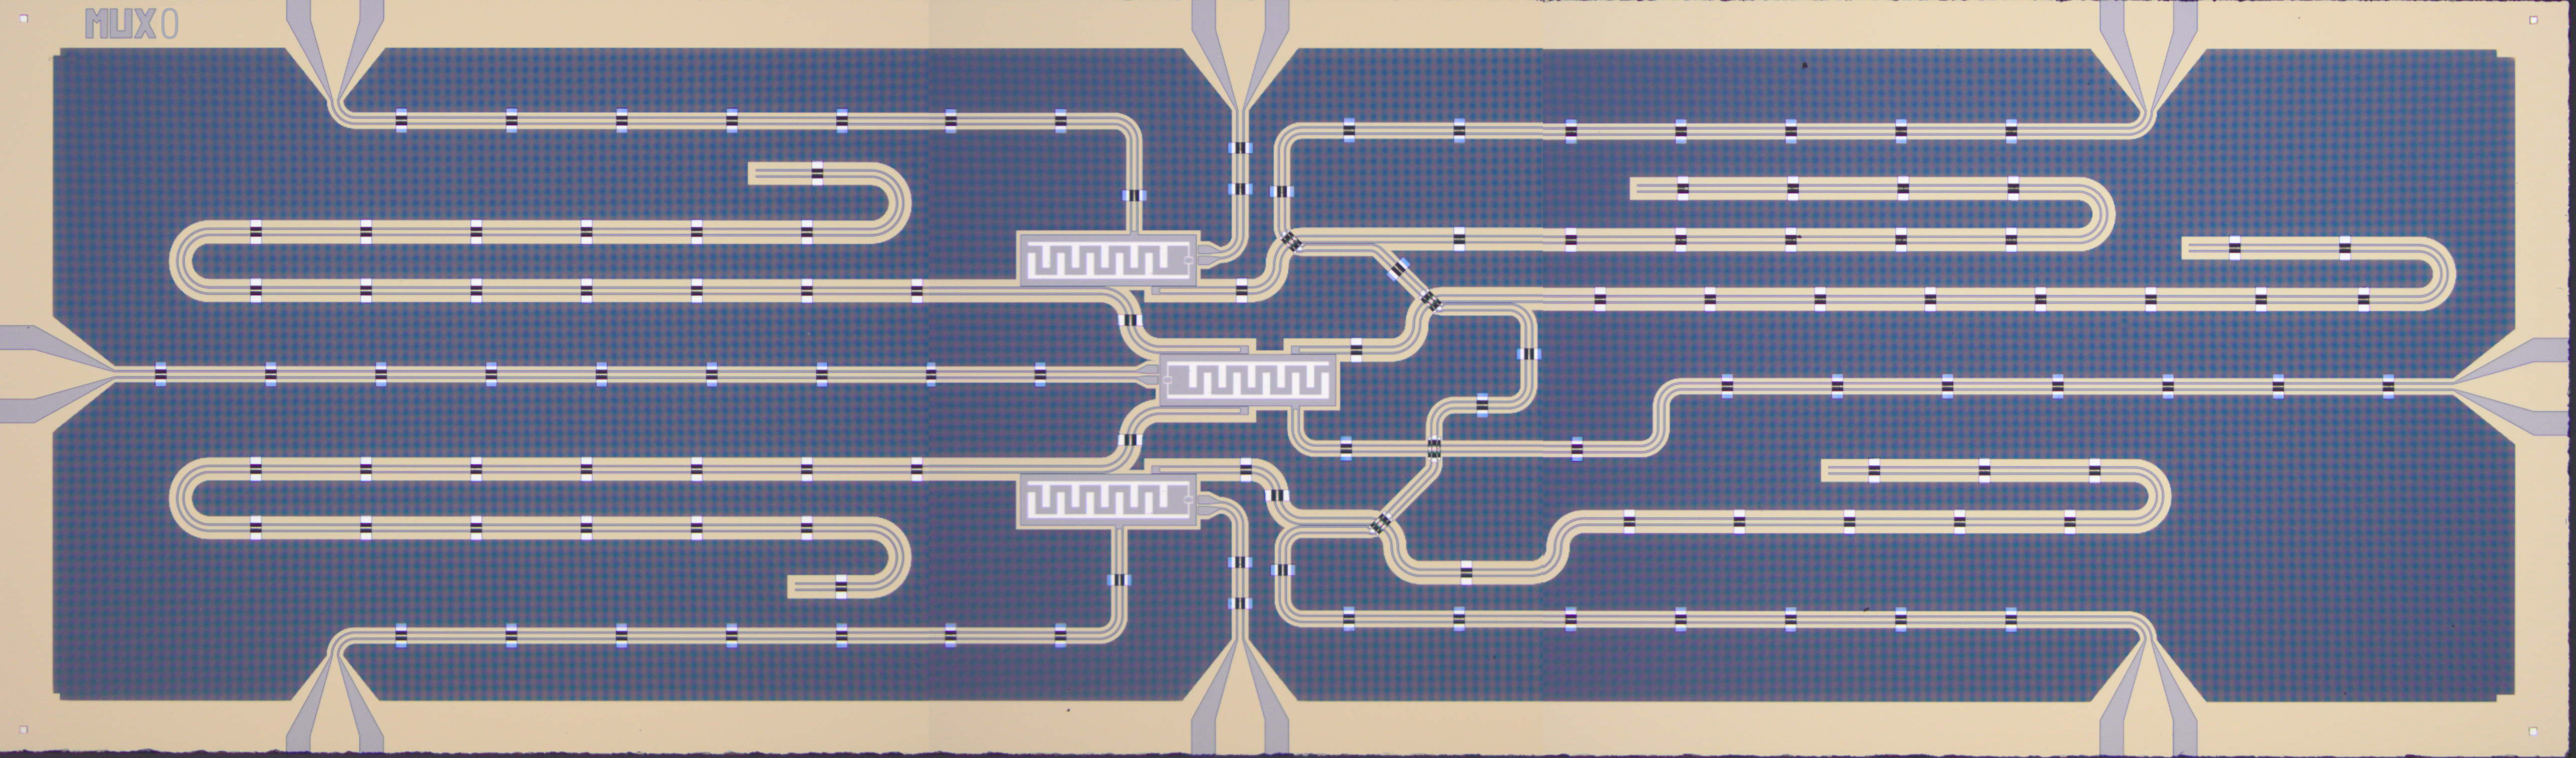
\includegraphics[width=1\linewidth]{../Figures/MUX_0.jpg}
          \caption{Muxmon0}
          \label{fig:Muxmon0 image}
        \end{subfigure}

        \begin{subfigure}[b]{0.9\textwidth}
          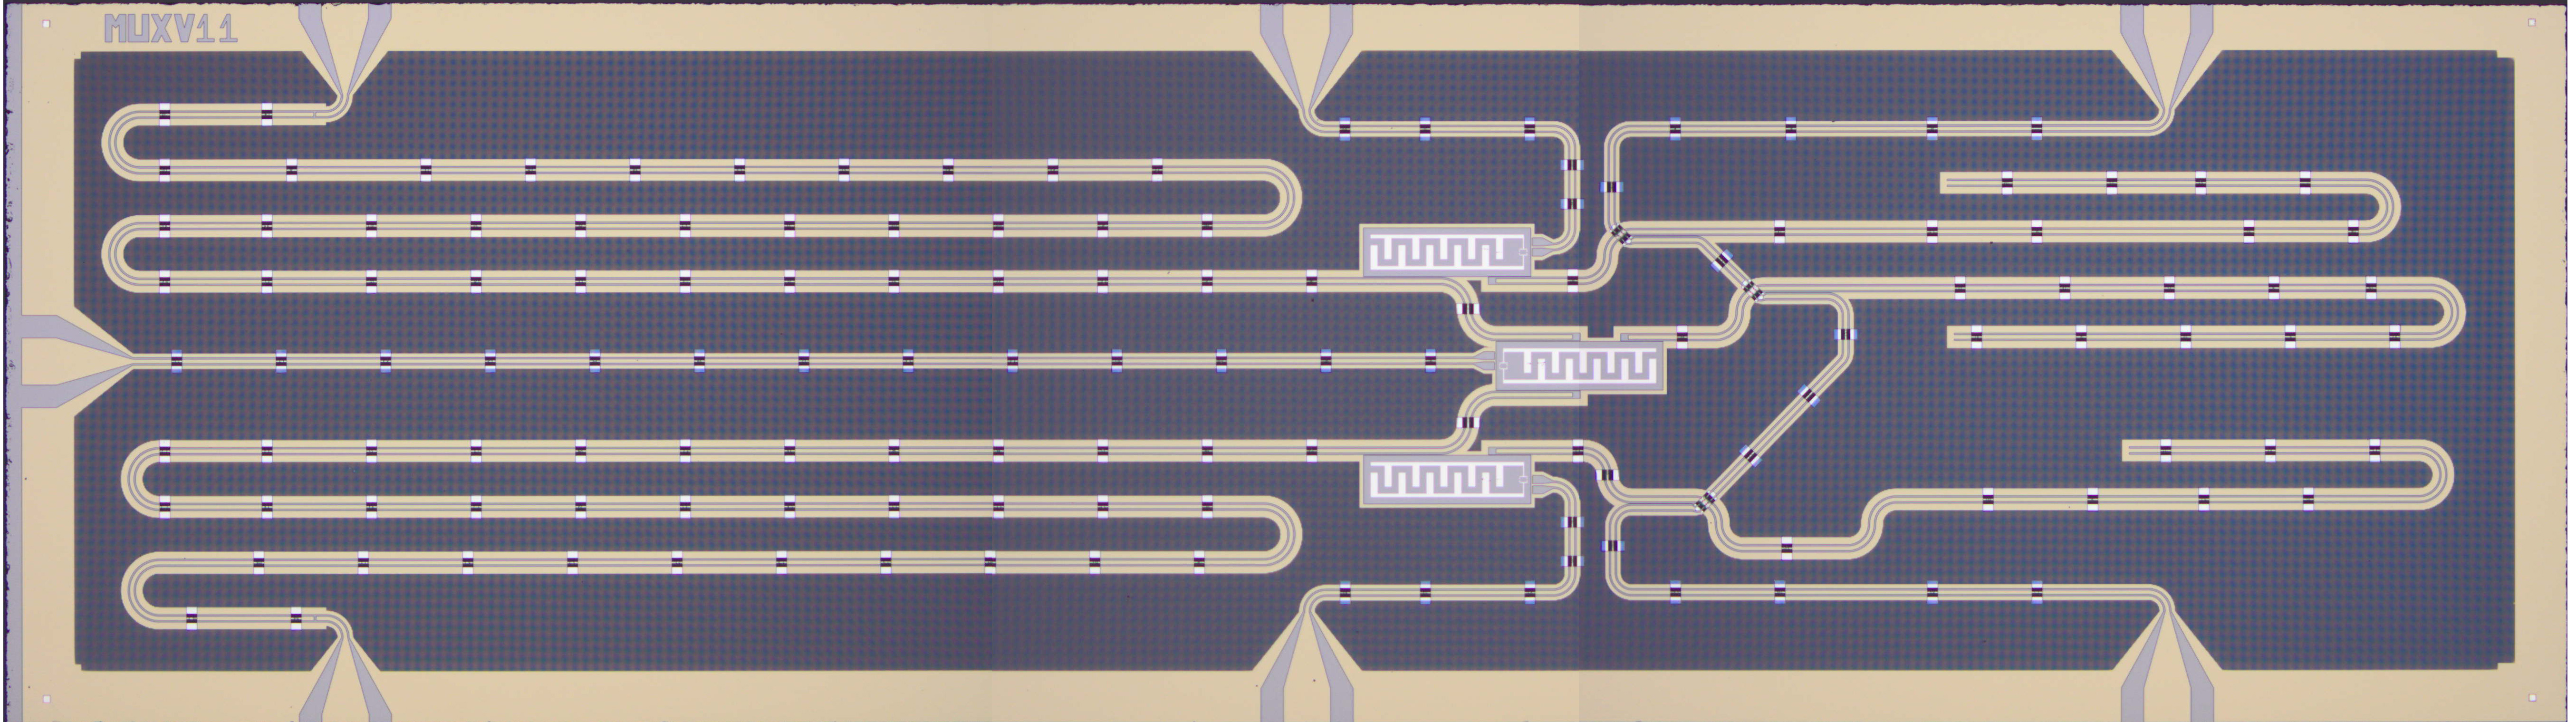
\includegraphics[width=1\linewidth]{../Figures/MUX_1.jpg}
          \caption{Muxmon1}
          \label{fig:Muxmon1 image}
        \end{subfigure}
        % \caption[Muxmon chips]{The Muxmon0 and Muxmon1 chips. The qubits of Muxmon0 have direct drive lines, whilst the }
        \label{fig:Muxmon0 and Muxmon1}
      \end{figure}

      The Muxmon0 and the Muxmon 1 chips were designed to study pulse multiplexing and frequency re-use. The two chips are shown in Figure~\ref{fig:Muxmon0 and Muxmon1}. Both chips have three transmon qubits connected to them, all three of which are flux-tunable. The key difference between the two chips is the approach used to drive the qubits In Muxmon0 all three qubits have their individual directly coupled drive lines. The top and bottom qubit are connected to the ancilla qubit through a bus. In the Muxmon1 the bus and drive lines are combined into two drive lines, each of which is capacitively coupled to the ancilla qubit and one of the other two qubits. The disadvantage of the direct drive lines in Muxmon0 is that they are an added decoherence channel for the qubits. However, the three drive lines of Muxmon0 ensure that individual qubit control of all three qubits is possible, even when they share the same frequency. This is in contrast to Muxmon1, where the ancilla qubit frequency must differ from that of the other two qubits. In the frequency re-use structure of the surface code, as explained in section\ref{sec:Frequency re-use in the Surface Code}, this should not be a problem, as frequency re-use in not applied to neighbouring qubits. Having capacitively coupled drive lines would result in less lines being required, both on-chip and outside the chip. Furthermore there would be one decoherence channel less. Therefore the capacitive coupled drive lines of Muxmon1 seemed the more attractive of the two options.

      During initial characterization of the qubits on both chips it was found that the coherence times of the qubits in Muxmon1 were considerably worse than those in Muxmon0. It is, however, unlikely that this is due to the capacitively coupled drive lines, since one would expect the absence of direct drive lines to result in one less decoherence channel. Instead it is likely that the lower coherence times are simply due to some error in the chip fabrication process. Due to the lower coherence times of the qubits in Muxmon1, the focus of the experiment was on Muxmon0.

      \textbf{TODO:}
      \begin{itemize}
        \item Mention correct coherence times.
      \end{itemize}

    \section{Properties of the Muxmon0 chip}

      \begin{figure}[tb]
        \centering
        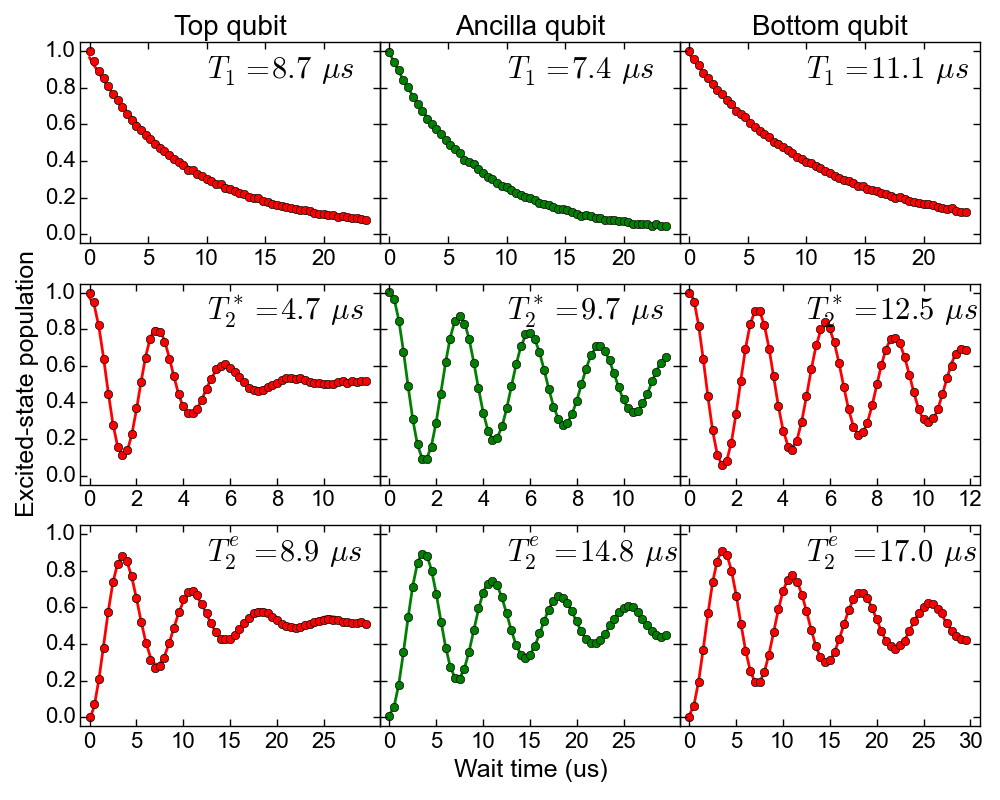
\includegraphics[width=\linewidth]{../Figures/Exploring frequency re-use/coherence_times.png}
        \caption{Coherence times of the three qubits in Muxmon0. The top qubit frequency is tuned to match the bottom qubit frequency (\SI{6.22}{\giga \hertz}).}
        \label{fig:coherence times Muxmon0}
      \end{figure}

      \begin{table}
        \begin{tabular}{l || c | c | c}
          Qubit  & $f_\text{max}$ (GHz) & $f_\text{res}$ (GHz) & coupling strength $g$ \\
          \hline
          Top    & 6.277                & 6.700                & ?\\
          Ancilla& 6.551                & 6.733                & ? \\
          Bottom & 6.220                & 6.800                & ?
        \end{tabular}
        \caption{Sweet-spot frequencies $f_\text{max}$, resonator frequencies $f_\text{res}$ and coupling strengths $g$ of the three qubits in the Muxmon0 chip}
        \label{tab:Muxmon0 qubit properties}
      \end{table}
      In the Muxmon0 chip the top and bottom qubits are each coupled to the ancilla qubit via a resonator bus. The frequencies of the qubits and their corresponding resonators are shown in Table~\ref{tab:Muxmon0 qubit properties}. All three qubits are operating in the dispersive regime, as the minimum detuning is considerably larger that the coupling strength for all qubits.

      To study frequency re-use, the top qubit frequency has been tuned to that of the bottom qubit, while the ancilla and bottom qubits were kept at their respective sweet-spots. Under these conditions the coherence times of the three qubits are shown in Figure~\ref{fig:coherence times Muxmon0}. The dephasing time $T_2^*$ of the top qubit is considerably worse than of the ancilla and bottom qubit. This is because the top qubit has been tuned away from its sweet-spot, and so is more susceptible to flux noise.

      \textbf{TODO:}
      \begin{itemize}
        \item explain top ancilla and bottom qubit
        \item find coupling strengths
        \item  The fit to $T_2^*$ of the top qubit has been performed using a Gaussian noise model.
      \end{itemize}

    \section{Cross-coupling}

      \begin{figure}[tb]
        \centering
        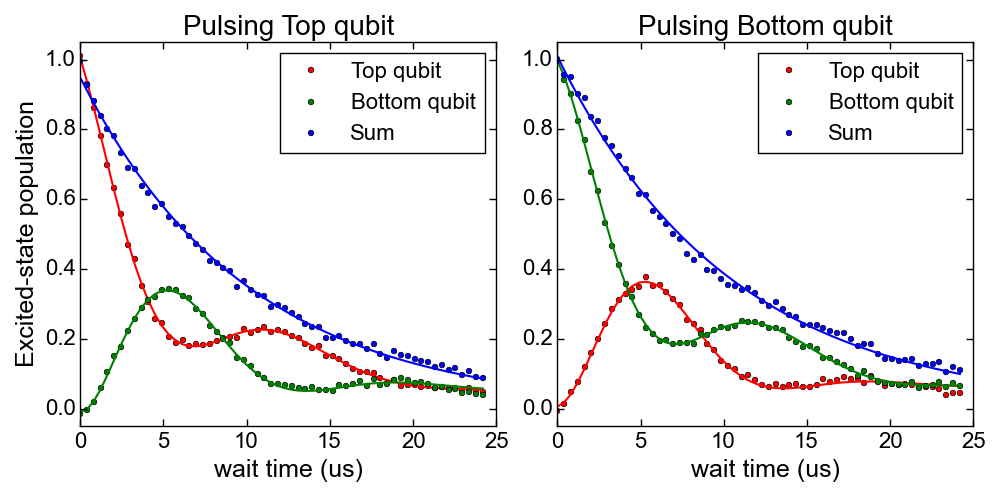
\includegraphics[width=\linewidth]{../Figures/Exploring frequency re-use/excitation_swap.png}
        \caption{After initially exciting one qubit, and measuring the excited-state population of both qubits versus time, an excitation swap is observed. The extracted coupling strength is equal to $J2\pi=72.0 \pm 1.8$ kHz}
        \label{fig:excitation swap}
      \end{figure}

      The top qubit is coupled to the botom qubit via the following three successive components:

      \begin{enumerate}
        \item The resonator bus coupling the top qubit to the ancilla qubit.
        \item The ancilla qubit.
        \item The resonator bus coupling the two ancilla qubit to the bottom qubit.
      \end{enumerate}

      When the top and bottom qubit are tuned into resonance, the two qubits experience an exchange interaction. This interaction leads to an excitation in one qubit being able to travel to the other qubit. This can result in the swapping of excitation between the top and bottom qubit, at a rate given by the interaction strength $J$. The excitation swapping of the top and bottom qubit when tuned into resonance can be seen in Figure~\ref{fig:excitation swap}. From these results the coupling $J$ is found to be equal to $J/2\pi=72. \pm 1.8$ kHz. For more information on the exchange interaction see section~4.3.2 of the thesis by Chow \cite{Chow}.

    \section{Cross-driving}
      \label{sec:cross-driving}

      {\centering
        \begin{minipage}{0.65\textwidth}
          \centering
          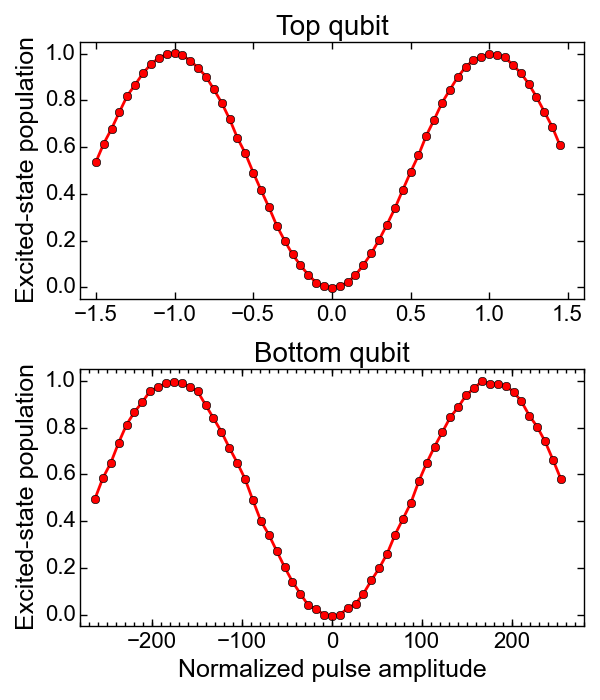
\includegraphics[width=\textwidth]{../Figures/Exploring frequency re-use/cross-driving_Rabi.png}
          \captionof{figure}{Required drive amplitude required to drive the top and bottom qubit through the top qubit drive line. The amplitude has been normalize to the amplitude required for a pi pulse on the top qubit.}
          \label{fig:cross-driving Rabi}
        \end{minipage}
        \begin{minipage}{0.35\textwidth}
          \centering
          \begin{tabular}{c | c}
            qubit & cross-driving (\%) \\
            \hline
            Top & $100$ \\
            Ancilla &$ 0.79$ \\
            Bottom & $0.57$
          \label{tab:cross-driving top}
          \end{tabular}
          \captionof{table}{Driving through top qubit drive line}
          \vspace{2cm}
          \begin{tabular}{c | c}
            qubit & cross-driving (\%) \\
            \hline
            Top & $0.23$ \\
            Ancilla &$ 0.66$ \\
            Bottom & $100$
          \end{tabular}
          \captionof{table}{Driving through bottom qubit drive line}
          \label{tab:cross-driving bottom}
        \end{minipage}
      \vspace{1cm}
      }

      When driving one of the qubits through its dedicated drive line, the signal can partially leak through to the other qubits. The cause of this leakage may be on-chip, where the components separating the qubits do not fully filter the signal, or may be off-chip, due to for instance imperfect isolation between the cables or other components. This signal leakage results in cross-driving effect, where driving one qubit will also partially drive the other qubits.

      \begin{figure}[tb]
        \centering
        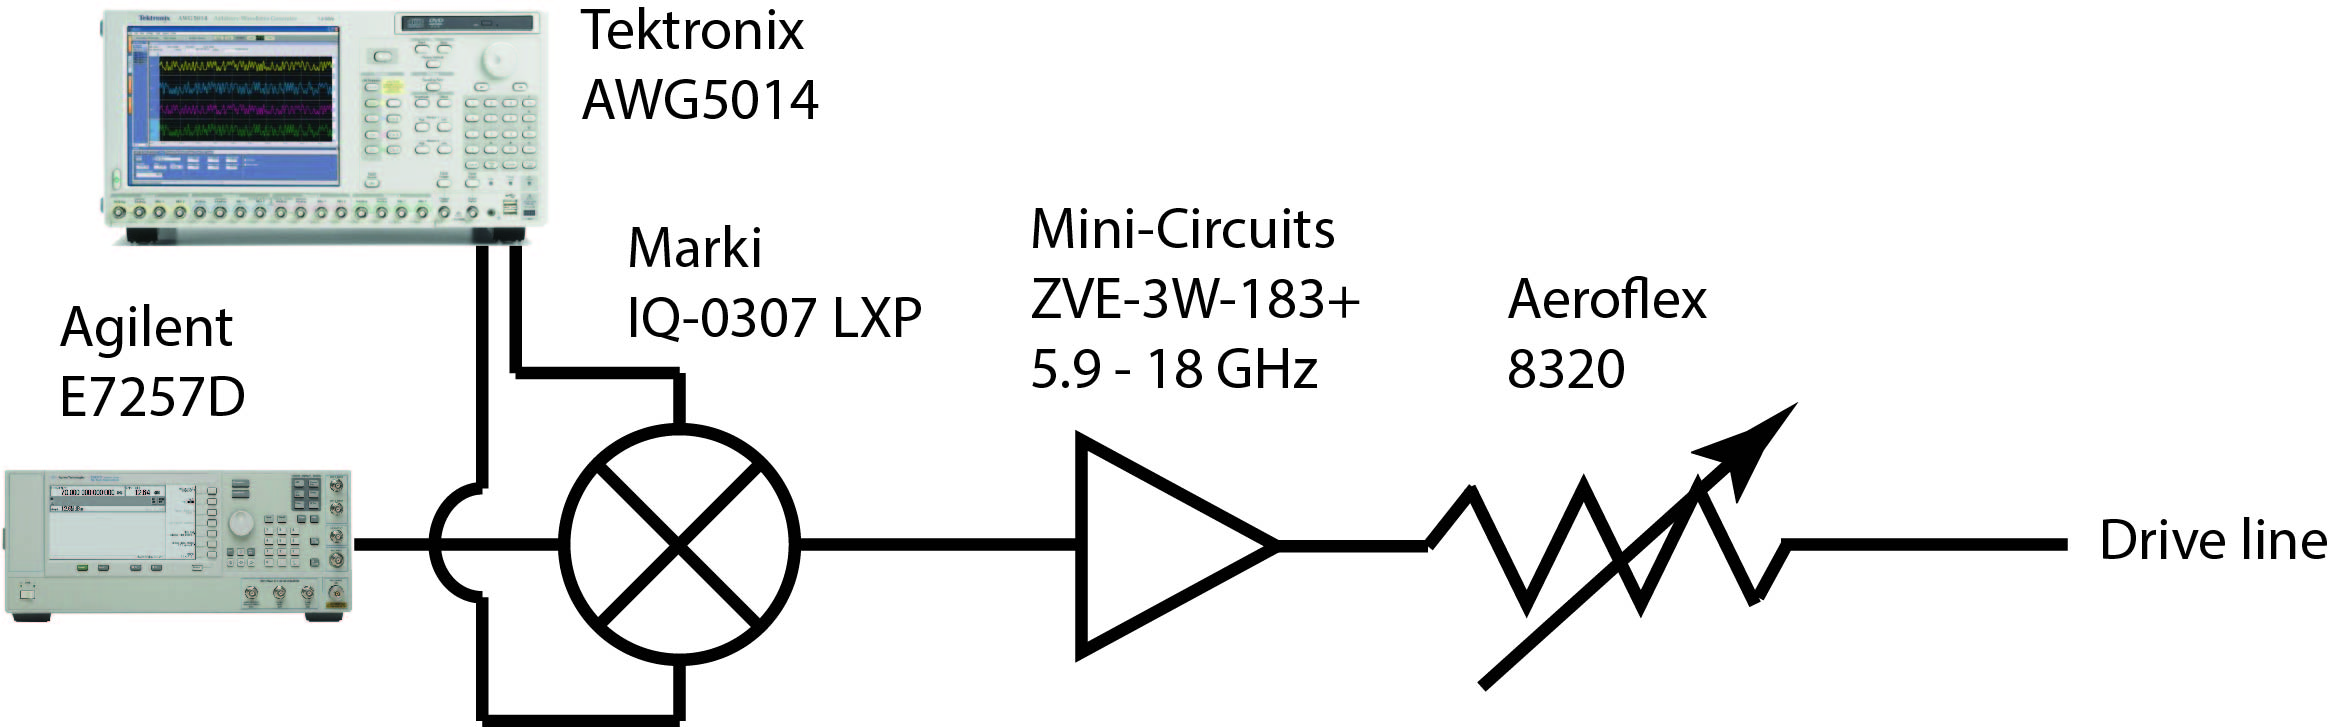
\includegraphics[width=.8\textwidth]{../Figures/Exploring frequency re-use/cross-driving_setup.jpg}
        \caption{Schematic for measuring the amount of cross-driving using the direct drive lines of the top and bottom qubit.}
        \label{fig:cross-driving schematic}
      \end{figure}

      The amount of cross-driving can be determined by measuring the pulse amplitude required to drive each of the three qubits through a drive line. The cross-driving due to the finite isolation of the Duplexer has been separately measured (see Appendix~\ref{ch:Duplexer isolation}). At the frequencies used in the experiment, the isolation of the Duplexer was found to be typically around \SI{50}{\dBm}. The amount of cross-driving due to other sources was determined by measuring the pulse amplitude required to perform a Rabi on each of the qubits using a fixed drive line. The measurements were performed using the set-up shown in Figure~\ref{fig:cross-driving schematic}. The results of a single cross-driving measurement is shown in Figure~\ref{fig:cross-driving Rabi}, where the top and bottom qubit are driven through the drive line of the top qubit. The pulse amplitude is normalized to the amplitude required for applying pi pulse to the qubit directly connected to the drive line. The amount of cross-driving is equal to the ratio of the pulse amplitude required for a pi rotation for the main qubit, and for the cross-driven qubit. The cross-driving ratio's are shown in Tables~\ref{tab:cross-driving top} and ~\ref{tab:cross-driving bottom}. The cross-driving ratio's are found to be less than one percent, and are higher for the ancilla qubit than for the other cross-driven qubit. This indicates that the main source of cross-driving is likely on-chip. Furthermore it can be seen that the cross-driving is stronger from the drive line of the top qubit than from the drive line of the bottom qubit.

      \begin{figure}[tb]
        \centering
        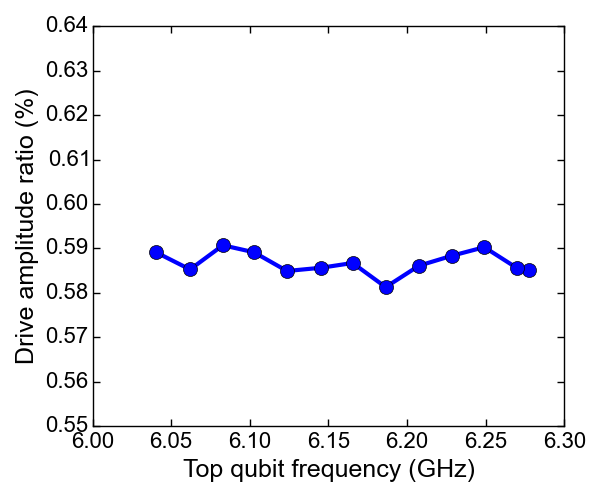
\includegraphics[width=.5\textwidth]{../Figures/Exploring frequency re-use/cross-driving_vs_top_frequency.png}
        \caption{Cross-driving ratio of the bottom qubit when pulsing from the drive line of the top qubit, versus frequency of the top qubit. }
        \label{fig:cross-driving versus top frequency}
      \end{figure}

      As a check that the effects observed are indeed due to cross-driving, and not due to cross-coupling, the cross-driving when driving the bottom qubit through the drive line of the top qubit has been measured as the frequency of the top qubit is varied. The results are shown in Figure~\ref{fig:cross-driving versus top frequency}. If the effect is due to cross-coupling the amount of cross-driving should depend strongly on the detuning between the top qubit and bottom qubit. Instead we see that the cross-driving is approximately constant, indicating that this is indeed a cross-driving effect instead of a cross-coupling effect.



    \textbf{Topics that should be explained in this section:}
    \begin{itemize}
      \item Explain similarities of chips
      \begin{itemize}
        \item Air bridges are used, not only for connect the ground planes, but also such that the feed line can pass over other coplanar waveguides without contact \\
      \end{itemize}

      \item Explain differences between Muxmon0 and Muxmon1.
      \begin{itemize}
        \item The Muxmon0 chip has a driving line connected to each of the qubits. \\
            It has two resonator buses at \SI{4.9}{\giga \hertz} and \SI{5.0}{\giga \hertz}. \\
            These could also be used for two-qubit gates.
        \begin{description}
          \item[Advantage] Able to fully control each qubit individually, even when multiple qubits share the same frequency.
          \item[Advantage] Less coupling between data qubits.
          \item[Disadvantage] Requires more driving lines.
          \item[Disadvantage] Adds extra source of dissipation for the qubits.
        \end{description}
        \item The Muxmon1 chip has two driving lines, each capacitively coupled to one of the two data qubits, and to the ancilla qubit.
        \begin{description}
          \item[Advantage] Less driving lines required
          \item[Advantage] Less dissipation due to capacitive coupling
          \item[Disadvantage] Cannot individually control data qubit and ancilla qubit when they share the same frequency
          \item[Disadvantage] More coupling between qubits
        \end{description}
        \item Simplified model of the surface code
      \end{itemize}

      \item Explain concepts of cross-coupling and readout cross-talk
      \begin{description}
        \item[Cross-coupling] The coupling between qubits. \\
                    Cross-coupling leads to transfer of excitation.\\
                    An associated coupling strength \textbf{g} can be associated to cross-coupling.\\
                    Can be determined by driving one qubit extremely hard, and measuring signal from other qubit.\\
                    \textbf{TODO:} Show values of cross-coupling found, or do this in characterization section \\
                    \textbf{TODO:} Leads to coherent errors? \\
                    \textbf{TODO:} Two types of cross-coupling? Direct leakage of pulse pulse, and transfer of excitation? cross-driving?
        \item[Readout cross-talk] Coupling between a qubit and a resonator that are not directly coupled.\\
                      A part of the signal measured from one resonator is then due to the state of another qubit \\
                      \textbf{TODO:} Understand more behind readout cross-talk
      \end{description}

    \end{itemize}

    \textbf{Left to think about:}
    \begin{itemize}
      \item Should I already include items such as coherence times, the fact that Muxmon0 performs better than Muxmon 1?
      \item Where should I include coherence times versus frequency?
      \item Should the part on cross-coupling and readout cross-talk not be in characterization section?
      \item Should the section on the Duplexer go in here?
    \end{itemize}

    \textbf{Figures that need to be included:}
    \begin{itemize}
      \item Muxmon0 and Muxmon1 chip, preferably optical microscopy
      \item SEM image of air-bridges such that coplanar wave-guides cross without intersecting
      \item schematic of cross-coupling and readout cross-talk \\
          It could be good to create this using the actual Muxmon chip as background, with arrows indicating how the different effects operate
    \end{itemize}


  \chapter{Randomized benchmarking}

    \section{Second excited state}

  \chapter{Conclusions and outlook}
